\documentclass[12pt]{article}

%设置页边距
\usepackage{geometry}
\geometry{left=2.5cm,right=2.5cm,top=2.5cm,bottom=2.5cm}

%地址链接支持
\usepackage{hyperref}

%支持分栏
\usepackage{multicol}

%页眉页脚
\usepackage{fancyhdr}
\pagestyle{fancy}
\lhead{项目进展报告}
\rhead{Project Progress Report}

%设置字体
\usepackage[no-math]{fontspec}
\usepackage{xunicode}
\usepackage{xltxtra}
\setmainfont[AutoFakeSlant]{Hiragino Sans GB W3}

%设置换行缩进
\usepackage[indentfirst=false,slantfont,boldfont]{xeCJK}
\usepackage{indentfirst}
\setlength{\parindent}{0.9cm}

%行距
\linespread{1.2}

\begin{document}

\title{项目进展报告:\\[3ex] 基于主页标题文字的\\热点新闻跟踪与分析、可视化展示\\[3ex]}

\author{郭志芃\quad\href{mailto:gzp9595@gmail.com}{gzp9595@gmail.com}\\
	徐磊\quad\href{mailto:leopard.lie@gmail.com}{leopard.lie@gmail.com}\\
	张宇翔\quad\href{mailto:zz593141477@gmail.com}{zz593141477@gmail.com}\\[3ex]}
\date{2014年5月10日}
\maketitle
\newpage
\renewcommand{\contentsname}{项目进展报告}
\tableofcontents
\newpage
\section{简介}
“基于主页标题文字的热点新闻跟踪与分析、可视化展示”这一项目需要实现的功能为:对各大门户网站的新闻进行整合,将结果以一种优雅的方式展示给用户。由于新闻标题往往都包含了很大的信息量,同一事件的新闻标题也存在大量相同的词语,所以从统计学意义上对新闻标题进行处理就能很好的对标题进行整合。我们组计划前期将只支持某些特定的网站,未来有可能对用户指定的URL提供支持。
\section{分工}
\begin{center}
\begin{table}[!hbp]
\begin{tabular}{||l|l||}
\hline\hline
对网页新闻标题的抓取及存储 & 张宇翔\\
\hline
对新闻标题的分析处理 & 徐磊\\
\hline
对处理结果的可视化展示 & 郭志芃\\
\hline\hline
\end{tabular}
\end{table}
\end{center}
\section{设计说明与进度}
\subsection{抓取}
网页抓取是整个系统的主要数据源,其准确性与可扩展性直接影响后期处理的效果,而现在各种web技术纷繁多样,导致抓取变得困难.因此这部分的设计充分利用了OOP中继承的优势,减少冗余代码,提高可扩展性.

本部分集成了html和json解析,能够适应大部分的web页面和ajax请求数据解析,尽可能多的支持各个新闻网站.

主要类的设计如下:

\begin{itemize}
\item SpiderBase\\
所有Spider的基类,提供网页抓取的基础功能(如HTTP请求,编码转换)及异步任务调度,目前仅实现了前者

\item GumboBasedSpider\\
提供基于第三方库gumbo的html dom树解析,类中声明了两个纯虚的回调函数,留给子类实现,以适应不同网站的不同网页结构.
其中searchNodeCallback在递归遍历dom节点时调用,由子类判断节点是否有用,是否需要深入遍历;resultCallback在遍历先前存储的节点时,有子类进一步过滤出需要保留的信息.

\item JsonBasedSpider\\
提供对于json格式数据的解析,尚在开发中.

\item SpiderFor163,SpiderForQQ,SpiderForSina\\
继承自SpiderBase,GumboBasedSpider,提供对于门户网站新闻主页的抓取

\item SpiderFor163,SpiderForSinaRoll\\
继承自SpiderBase,GumboBasedSpider,提供对于门户网站滚动新闻的抓取

\item SpiderForQQRoll\\
继承自SpiderBase,GumboBasedSpider,JsonBasedSpider,提供对于提醒滚动新闻的抓取.由于腾讯滚动新闻采用ajax加载包含html的json的机制,使得该功能必须同时依赖两种解析器.
\end{itemize}

\subsection{存储}
本系统提供历史新闻跟踪分析功能,要求存储历史抓取数据,因此设计了数据存储部分.为了快速查找,这部分使用数据库作为后端存储.目前选用的轻量级的关系型数据库sqlite,如有必要,后期可考虑选用文档性数据库(NoSQL)实现更加灵活的数据存储.

主要类的设计如下:

\begin{itemize}
\item StorageBase\\
提供与数据库引擎无关的数据操作接口,使主程序与数据库解耦.目前,仅实现了插入和按日期查找的接口.

\item SqliteDatabaseStorage\\
继承自StorageBase,实现接口数据类型向sqlite数据库的类型转换,以及sql语句构造等功能.
\end{itemize}

\subsection{分析}
分析部分需要实现将一个大的标题列表分成若干类的功能,需要解决的问题是分类的数量和分类的标准。目前已经实现的算法都基于一个假设,就是每个标题应当属于且仅属于一个分类。为了方便表述,我们把标题的列表称为$L$,把分类后的结果称为$S$,具体的说,$S$的每个元素是一个分类,而分类是一个标题的集合。基于之前的假设可以表述为$(\forall x \in L)(\exists u \in S)((x \in u )\bigwedge(\forall v \in S) (x \in v \Rightarrow u = v))$,作出形式化的描述只是为了将符号的含义解释清楚,对后面的算法并没有什么作用。

一种分析的方法是以字为单位进行的。对$L$中的每个标题$x$分别处理,计算$x$与$S$中每个已有分类$u$的相似度,如果各个分类相似度的最大值大于某个阈值,则将$x$放入取得最大值的分类$u_0$,否则将$\lbrace x\rbrace$作为一个新的分类加入$S$中。现在需要定义一下相似度,将标题$x$与$y$的相似度定义为$y$中字符在$x$中出现的数量除$y$的长度,$x$与分类$u$的相似度定义为$x$与$u$中各个标题相似度的代数平均。实践表明,在阈值设定为0.2时可以得到较好结果。这种方法的优点在于分类的数量是动态的,分类的标准时可控的,但是相似性的计算粗糙导致结果不好。

另一种分析的方法是以词为单位进行的。在已有算法中采用双向最大匹配算法进行分词,运用自然语言处理中常见的TF-IDF的方法对每个词给予了一定的权重。每个标题看做一个高维的向量,每个维度就表示一个次的TF-IDF值,运用cos-similarity来评估两个向量的相似性。最后运用K-means算法对向量进行聚类。这样做的优点在于减少了一些在标题中广泛使用的词语对结果的影响,K-means在聚类算法中得表现也较为优秀。缺点是手动确定分类数量需要超凡的技巧。

在实现上述算法的过程中,使用了很多面向对象的思想。在实现算法之前,先定义好了接口,以及$L$和$S$的类型,使得前处理和后处理都能同步的进行,在类型的定义中,预留了一些特性来增强可扩展性。两种算法都是同一基类的派生类,所以用法相对一致,更换算法不需要对主程序进行大的修改。在第二个算法实现过程中,需要用到Trie这一数据结构,在此复用了之前写过的模板,模板的使用使得这个代码可以适用于string、u32string、int等各种类型的容器,代码的复用避免了“重新发明轮子”。
\subsection{展示}
我们在展示方面,想过很多方法,最后想用的是html+javascript进行展示。这两个不仅可以很好的展示出来树状结构,更有很多特效可以将我们要的重点突出出来。关于怎么实现html,我们使用C++中的一个第三方库:microhttpd。它相当于在电脑上实现一个本地服务器。
在html上,我们准备将所有的关键词呈现出来,让用户进行选择,然后我们将和这些选择的关键词有关的新闻标题凸显出来,这些标题是以时间顺序呈现出来,并且提供用户进行点击查看网页。

\subsection{UML}
\begin{center}
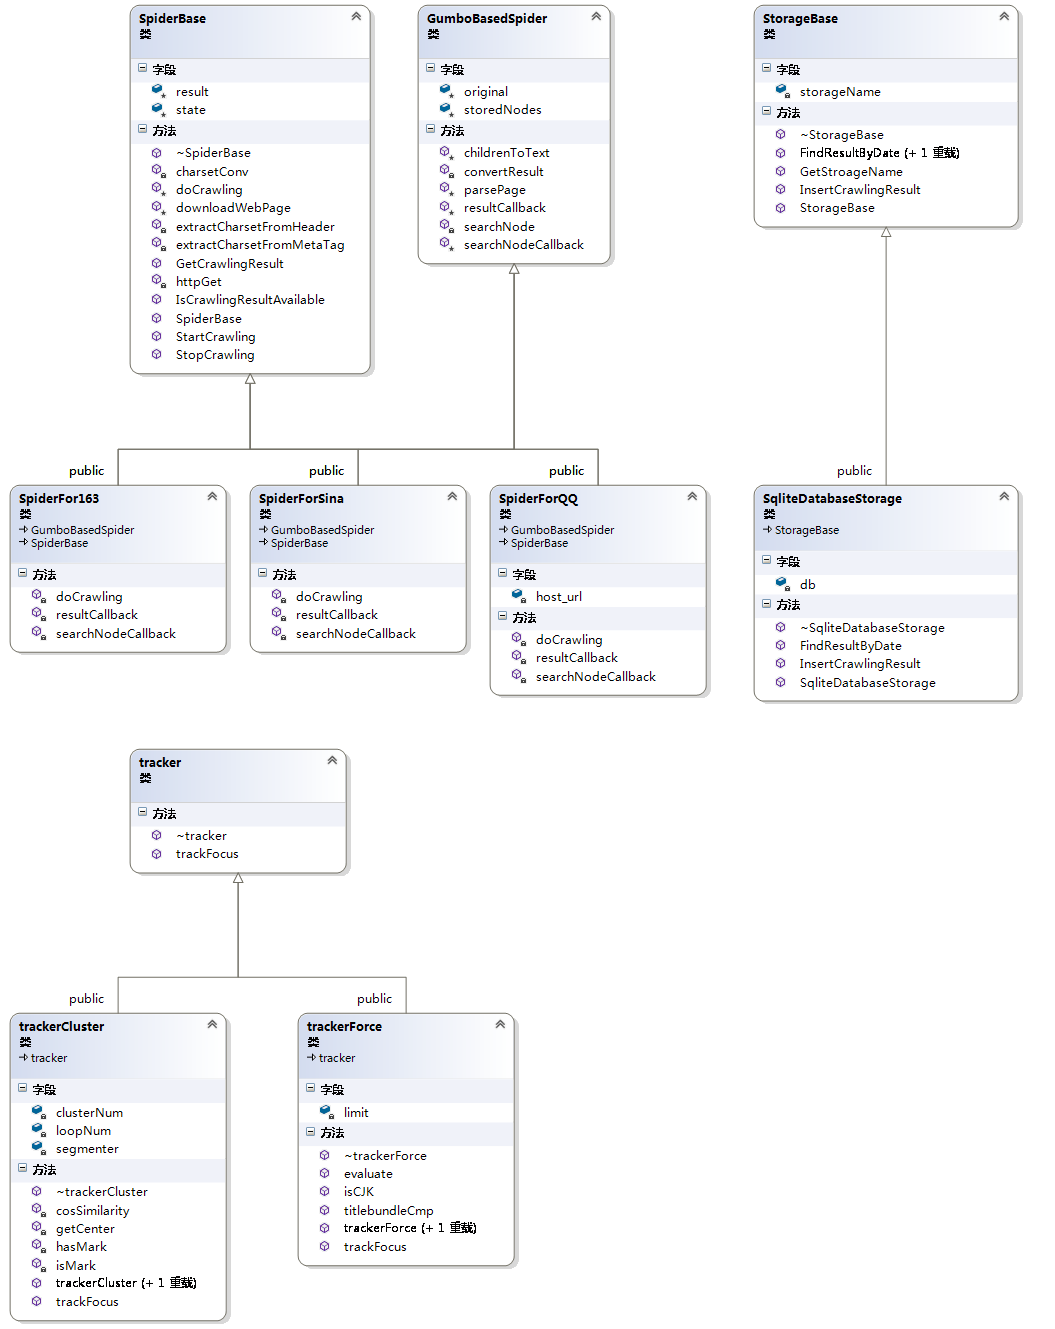
\includegraphics[width=\textwidth]{midUML.png}
\end{center}
\section{目标}
抓取部分,完成json解析类.由于大部分现有的json库都不支持一些非标准json语法(而某些网站又使用了它们),准备使用flex+bison生成词法/语法分析器,实现自己的json解析器.

数据存储部分,配合UI端设计更多的查询接口.
\end{document}